\begin{abstract}
Movement primitives (MPs) provide a powerful framework for data driven movement generation that
has been successfully applied for learning from demonstrations and robot reinforcement learning. 
In robotics we often want to solve a multitude of different, but related tasks. As the parameters of the primitives are typically high 
dimensional, a common practice for the generalization of movement primitives to new tasks is to 
adapt only a small set of control variables, also called meta parameters, of the primitive. Yet, for most MP representations, the encoding
of these control variables is pre-coded in the representation and can not be adapted to the considered tasks. 
In this paper, we want to learn the encoding of task-specific control variables also from data instead of relying on fixed meta-parameter representations. 
We use hierarchical Bayesian models (HBMs) to estimate a low dimensional latent variable model 
for probabilistic movement primitives (ProMPs), which is a recent movement primitive representation. We show on two real robot 
datasets that ProMPs based on HBMs outperform standard ProMPs in terms of generalization and learning from a small amount of data 
and also allows for an intuitive analysis of the movement. We also extend our HBM by a mixture model, such that we can model 
different movement types in the same dataset. 
\end{abstract}

\section{Introduction}

Movement primitives (MPs) are a compact parametric description of a movement
\cite{Paraschos2013,Ijspeert2003,Khansari-Zadeh2011,dAvella2003}. They provide a powerful framework for 
data driven movement generation as they can be learned from demonstrations as well as by reinforcement learning. They can adapt
to a new task by adapting a given set of meta-parameters
\cite{Ude2010,Kober2010, Kupcsik2013}. For example, the final joint positions or the execution speed \cite{Ijspeert2003} of the movement can be adapted. 
%\begin{figure}
\begin{wrapfigure}{r}{0.4\columnwidth}
%\vspace{-0.5em}
\begin{center}
\includegraphics[width=0.38\columnwidth]{elmarICRA/pics/IMG_1062_mod2.JPG}
\end{center}
\caption{The robot used in the experiments to learn trajectory distributions.}
\vspace{-1.5em}
%\end{figure}
\end{wrapfigure}
Yet, for most movement primitive representations, the 
set of meta-parameters is pre-coded into the movement primitive representation and can not be adapted. However, for most tasks, a different encoding of the meta-parameters
might be more appropriate than the pre-coded parameters of the primitive representation. We believe that this shortcoming has 
also hindered the application of movement primitives for more complex multi-task learning applications. In this paper we want to 
learn the encoding of the meta-parameters also from data. Our approach extracts a low-dimensional manifold in the MP parameter space. Each point 
on this manifold is described by a small set of control variables. Hence, our underlying assumption is that, while the parametrization of 
movements might be high-dimensional, useful parameter vectors for a given set of tasks typically share a lot of structure, i.e. they lie on a lower dimensional manifold.
Each demonstration can now be characterized by the corresponding 
control variables that can be seen as a compact description of the task considered in this demonstration. For example, in a table tennis scenario,
these control variables could specify the location of the hitting point or the desired return direction for the ball. 
Hence, our model can not only be applied for efficient generalization in multi-task learning with movement primitives but is also well suited 
for analyzing the movements of human demonstrators. We represent the latent manifold model by a hierarchical Bayesian model. The control
variables for each demonstrations are treated as latent variables that are also inferred from the data. The model 
is extended by a mixture model such that we can learn the control variables of multiple types of movements. We will use 
Probabilistic Movement Primitives (ProMPs)  as underlying movement primitive representation as they can be naturally integrated
in the Hierarchical Bayesian Model (HBM) representation. When learning or analyzing movement data, we have to deal
with several challenges, such as high-dimensionality, noise, missing data, partial observations, and the data can 
contain multiple modes that represent different types of movements. In order to deal with all these requirements, we 
apply a fully Bayesian approach where we integrate out all the estimated parameters of the model. In our experiments, we will
illustrate the improved generalization properties of our approach compared to the standard ProMP approach in the case of a small 
amount of training data and show how demonstrations can be easily analyzed and characterized by the extracted latent control variables. 




\subsection{Related Work}

Movement primitives can be categorized into trajectory-based
\cite{Ijspeert2003,Rozo2013,Paraschos2013} and state-based representations
\cite{Khansari-Zadeh2011}. In this paper
we will focus on trajectory based approaches as they are more commonly used and easier to scale up to higher dimensions. A common trajectory-based
approach are the dynamical movement primitives (DMPs). DMPs \cite{Ijspeert2003} are represented by a parametrized dynamical system that is given
by a linear point-attractor that is perturbed by a non-linear time dependent forcing function. The forcing function can be used to encode an arbitrary 
shape of the trajectory and the weights of the forcing function can be easily obtained from demonstrations by linear regression. One of the benefits
of the DMP approach is that it specifies a small set of meta-parameters. These meta-parameters include the final position of 
the movement, which is given by the point attractor, the final velocities, the execution speed, or the amplitude of the movement \cite{Kober2010a,Pastor2009,Ijspeert2003}. 
In multi-task learning with DMPs \cite{Kober2010,forte2012line,Kupcsik2013}, it is a common strategy to only adapt the meta-parameters 
due to the high dimensionality of the  weights of the forcing function. While DMPs have several more benefits such as stability, 
and the ability to represent stroke based and rhythmic movements, DMPs also have several limitations, such as that they can not represent optimal behavior in stochastic systems and the adaptation of the trajectory due to the meta-parameters is based on heuristics.
%, e.g., the outcome of a co-activation of DMPs or to continuously switch from one DMP to another is not predictable.
These issues have been addressed by the recently proposed Probabilistic Movement Primitives approach \cite{Paraschos2013,Paraschos2013a}. 
ProMPs estimate a distribution of trajectories instead of encoding 
single trajectories. The main benefit of the probabilistic representation is that we can use probabilistic operators such 
as conditioning for adaptation and a product of distribution for co-activating primitives. 
A distribution over trajectories also contains information on which time points are relevant for the movement, 
e.g., time points with small variance in the Cartesian end-effector space could denote task relevant via-points or targets.  
%A distribution over trajectories also contains 
%information on which time points are relevant for the movement, i.e. time points with small variance and which time points are 
%not relevant to achieve the task, i.e, time points with high variance of the joint positions. 
However, in difference to DMPs, ProMPs are lacking meta-parameters 
that can be used to adapt the trajectories with a small amount of control variables. While it would be easy to pre-specify such control variables by 
conditioning the trajectory distribution for a fixed set of time points, such an approach would again require a lot of manual tuning and is lacking flexibility. 

Our approach automatically extracts a small amount of control variables from a given set of demonstrations in the ProMP framework. 
We use a hierarchical Bayesian approach to model prior distributions, which is inspired by techniques from multi-task learning (MTL) \cite{yu05,lazaric10,daume12,ruvolo14}.
In MTL the underlying assumption is that multiple tasks (or trajectories) share a common structure, and, hence, with 
an increasing number of related tasks that have been already learned, the number of needed training samples for generalizing to a new task decreases \cite{baxter00}. 
%The main advantage of learning multiple related task together is the increased the generalization performance by exploiting the shared information \cite{caruana97, baxter97} 
%which leads to a smaller amount of required training samples. 
This property is highly desired in robotics, where the data is often high dimensional and obtaining training samples is costly.
Different approaches exist to model the shared information across tasks. They can be roughly separated into two different categories, i.e. 
methods where parameters of the model are close to each other in a geometric sense \cite{evgeniou04,ruvolo14} and approaches 
where the parameters of the model share a common structure \cite{yu05,xue07,daume09,lazaric10,rai10,passos12}. 
This structure can be a clustering assumption \cite{xue07}, a (Gaussian) prior for the parameters of all tasks \cite{yu05,lazaric10} 
or some advanced structure like the Kingman's coalescent \cite{daume09}, which is a continuous time, partitioned valued Markov process. 
Our approach is highly related to the Bayesian MTL approach presented in \cite{passos12}, 
where a prior distribution over parameters is learned. 
The prior distribution is assumed to have a low-dimensional, latent structure that is represented by a linear factor model. In 
 order to represent several modes (or non-linearities) in the data, the model is extended to a mixture model of linear factor models.
 For both, the number of mixture components and the number of factors, a non-parametric Dirichlet prior has been used.
 All parameters of the model are integrated out by the use of a combination of sampling and variational inference. 
 We will use a simplification of this model, assuming a fixed number of mixture components, without the Dirichlet priors, 
 allowing a much more efficient algorithm without the need for expensive sampling methods. 
 We extend the model of Passos et al. by an additional hyper-prior and show that this hyper-prior significantly increases the robustness of the Bayesian model.
 
\section{Probabilistic Movement Primitives}

In this section we will give a brief overview on Probabilistic Movement Primitives (ProMPs) as they provide the foundation for our hierarchical Bayesian model. 
ProMPs represent a movement by a distribution $p(\vec \tau)$ over trajectories $\vec \tau = \vec y_{1:T}$, where $\vec y_t$ specifies the joint positions (or any other quantities, 
such as a Cartesian coordinates of a ball) at time step $t$. ProMPs use a linear basis function model with $J$ basis functions to represent a single trajectory, i.e.
$$ p(\vec y_t|\vec w) = \N \left (\vec y_t \middle |\vec \Psi_t \vec w,
\beta^{-1} \vec I \right ) \textrm{ and } p(\vec \tau) = \prod_{t=1}^T
p\left(\vec y_t\middle |\vec w\right),$$
where $\beta$ denotes the precision of the data. 
The weight vector $\vec w$  is a compact representation of the trajectory. 
The basis functions $\vec \Psi_t$ only depend on the time or, alternatively, 
on the phase of the movement. For a single Degree of Freedom (DoF), $\vec \Psi_t$ is just given by a vector of normalized Gaussian basis functions $\vec \phi_t$ with 
$$ \phi_{t,i} = \frac{\exp\left(-0.5 (t - c_i)^2 \right)}{\sum_{j = 1}^J \exp\left(-0.5 (t - c_j)^2\right)},$$
where $c_i$ denotes the center of the $i$th basis function (note that to enhance readability we skipped the bandwidth parameters in this notation).

For multi-dimensional systems with $D$ DoFs, the basis function matrix
is represented by a block-diagonal matrix, i.e, 
$$\vec \Psi_t = \left[\begin{array}{cccc} \vec \phi_t^T & \vec 0^T & \dots & \vec 0^T \\ \vec 0^T & \vec \phi_t^T &  \dots & \vec 0^T \\ \vdots & \vdots & \ddots & \vdots \\ \vec 0^T & \vec 0^T & \vec 0^T & \vec \phi_t^T  \end{array}\right].$$
Due to this encoding of the basis function matrix, the trajectories of all DoFs can still be represented as 
a single weight vector $\vec w^T = [\vec w_1^T, \vec w_2^T, \dots, \vec w_D^T]$ that is given by a concatenation of all 
weight vectors for each degree of freedom.

Still, a single weight vector $\vec w$ only represents a single trajectory $\vec \tau$. In order to represent a distribution over 
trajectories $p(\vec \tau)$, we can estimate a distribution $p(\vec w)$ over the weight vectors and, subsequently, integrate out the weight vectors. 
In the original ProMP approach, a multivariate Gaussian distribution is used to model the prior distribution 
\begin{align}\label{eq:priorProMPs}
p(\vec w) = \N(\vec w| \vec \mu_w, \vec \Sigma_w). 
\end{align}
As such, the distribution over trajectories is also Gaussian and can be computed in closed form 
\begin{align*}
 p(\vec \tau) & =  \int p(\vec \tau| \vec w) p(\vec w) d\vec w, \\
 & =  \int \N\left(\vec y_{1:T}\middle| \vec \Psi_{1:T} \, \vec w, \beta^{-1}
    \vec I\right)  \N\left(\vec w\middle| \vec \mu_w, \vec \Sigma_w\right) d\vec w,  \\
  & = \N\left(\vec y_{1:T}\middle| \vec \Psi_{1:T} \, \vec w, \vec \Psi_{1:T}
    \vec \Sigma_w \vec \Psi_{1:T}^T + \beta^{-1} \vec I\right),
\end{align*}
where $\vec \Psi_{1:T}$ is a $T D \times D J$ matrix containing the basis function matrices for all time steps 
and $\vec w$ is a $D J$ dimensional column vector.

\subsection{Learning from Demonstrations with ProMPs}

A ProMP already defines a simple hierarchical Bayesian model in a similar fashion as a Bayesian linear regression model. The mean $\vec \mu_w$ 
and the covariance matrix $\vec \Sigma_w$ can be learned from data by maximum likelihood using the Expectation Maximization (EM) algorithm \cite{Dempster1977}. 
A simpler solution that works well in practice is to compute first the most likely estimate of $\vec w^{[i]}$ for each trajectory $\vec \tau^{[i]}$ independently,
 where the index $i$ denotes the $i$-th demonstration\footnote{Given a trajectory $\vec \tau_i$, the corresponding 
weight vectors $\vec w^{[i]}$ can be estimated by a straight forward least squares estimate.}. 
Subsequently, mean and covariance of $p(\vec w)$ can be estimated 
by the sample mean and sample covariance of the $\vec w^{[i]}\,$'s. 
One advantage of the EM based approach in comparison to the more direct approach is that the 
EM algorithm can also be used for learning from incomplete data where, e.g., 
some segments of the trajectories might be missing due to occlusions in vision based recordings.
%\textit{Please note that ProMPs do not require the data to be sampled at uniform time intervals as the basis function matrix 
%can be computed for continuous points in time. I am not convinced that this feature is important for us.}

However, the training of ProMPs also suffers from a severe disadvantage. As the model has a lot of parameters due
to the high-dimensional covariance matrix, ProMPs suffer from overfitting if we have little training data and noisy trajectories. 
The more sophisticated hierarchical Bayesian model for ProMPs introduced in this paper alleviates this problem. 


%\begin{figure}
%\begin{center}
%\includegraphics[width=0.8\columnwidth]{PingPong_Data.png}
%\end{center}
%\caption{(A) Trajectory prediction task on a table tennis dataset. 
%The data consists of $20$ end-effector and ball trajectories illustrated in (B). 
%(C-E) Learned distributions over trajectories for three dimensions (out of six) using ProMPs. 
%The colors (red and blue) are only used to visualize differences in the movement directions.
%\label{fig:pingpong_data_promps}
%}
%\vspace{-0.5em}
%\end{figure}

%\begin{figure*}
%\begin{center}
%\includegraphics[width=0.8\textwidth]{PingPong_Overfitting.png}
%\end{center}
%\caption{The effect of noise (A) and missing data (B) on the prediction performance of ProMPs (blue lines) and LM-ProMPs (red lines).  
%In (A), from left to right the amount of applied noise to the data is increased. 
%In (B) four different frame rates of observations ($\in \{50, 100, 200, $ and $ 300\}$ms) are investigated.
%\label{fig:pingpong_overfitting}}
%%\vspace{-0.5em}
%\end{figure*}



\subsection{Predictions with ProMPs by Conditioning}

ProMPs can also be used to predict the behavior of the demonstrator once we have seen an initial part of a new trajectory. 
Lets assume that we have observed a human demonstrator at $m=1,2, ..., M$ different time points\footnote{Note that these time points do not need to be sampled in uniform time intervals.} 
$t_1$ to $t_M$ at the positions $\vec y_{t_1}$ to $\vec y_{t_M}$. 
Let us further denote $\vec \Psi_{\vec o}$ as the concatenation of the basis function matrices for these time points 
and $\vec o$ as concatenation of the $\vec y_{t_m}$ vectors. 
Given these observations,
we can obtain a conditioned distribution $p(\vec w| \vec o)$ over the weight vectors. 
This distribution is Gaussian with mean and variance
\begin{align}
\boldsymbol{\mu}_{\vec w| \vec o} & =  \boldsymbol{\mu}_{\vec w} + \nonumber \\ 
                                  & \boldsymbol{\Sigma}_{\vec w}\boldsymbol{\Psi}_{\vec o}^T\left(\boldsymbol{\Sigma}_o + \boldsymbol{\Psi}_{\vec o}\boldsymbol{\Sigma}_{\vec w}\boldsymbol{\Psi}_{\vec o}^T\right)^{-1}\left(\vec o -\boldsymbol{\Psi}_{o}\boldsymbol{\mu}_{\vec w}\right),  \label{eq:conditioningProMP1}\\
\boldsymbol{\Sigma}_{\vec w|\vec o} & =  \boldsymbol{\Sigma}_{\vec w}-\boldsymbol{\Sigma}_{\vec w}\boldsymbol{\Psi}_{\vec o}^T\left(\boldsymbol{\Sigma}_o +\boldsymbol{\Psi}_{\vec o}\boldsymbol{\Sigma}_{\vec w}\boldsymbol{\Psi}_{\vec o}^T\right)^{-1}\boldsymbol{\Psi}_{\vec o} \boldsymbol{\Sigma}_{\vec w}. 
\label{eq:conditioningProMP2}
\end{align}
%where the matrix $\boldsymbol{\Sigma}_o$ can be used to control the importance of different dimensions.% that is in the most simple case set to $\beta^{-1}\vec I$.
The conditional distribution  $p(\vec w| \vec o)$ can be used to predict the behavior of the demonstrator for future time points $t > t_M$, 
i.e. we can determine the mean and covariance of $\vec y$ for future time points. 
Note that the same procedure can be applied for partial observations, 
where only a subset of the quantities in $\vec y_t$ is observed. 
The covariance matrix $\boldsymbol{\Sigma}_o$ can be used to control the importance of different dimensions.
%(e.g., in our experiments we will condition on reaching a desired target in the Cartesian space using a KUKA robot arm without specifying the orientation of the end-effector, i.e, via $\boldsymbol{\Sigma}_o$). 

%\section{Hierarchical Bayesian Models for Probabilistic Movement Primitives}
\section{Extracting Control Variables with Hierarchical Priors}

Our goal is to model non-linear prior distributions that can be modulated by low-dimensional latent control variables. 
We define a hierarchical prior on the weight vector $\w$ using mixture models 
\begin{align}\label{eq:priorMixture}
  p(\wi) = \sum_{k=1}^K \pi_k \N\left(\wi\middle|\wok + \WVk \hki, \alpha^{-1}
      \vec I\right).
\end{align}
The vector $\wok$ denotes an offset term and the projection matrix
$\WVk$ defines the mapping from the low-dimensional control variables 
$\hki$ to the weight vector $\wi$ of trajectory $i$. The parameter
$\alpha$ models the precision of the latent manifold priors 
and $\pi_k$ denotes the mixing coefficients.
The different mixture components can model different movement types, e.g., forehand and backhand strokes in a table tennis game. 
Within a mixture component the latent control variable $\hki$ models the adaptation of 
the movement to the current task.

All parameters of this prior distribution are unknown a priori and are learned from demonstrations.  
We follow a fully Bayesian approach, where 
we treat all parameters as random variables and introduce conjugate priors for these random variables. We 
derive variational update equations for all relevant distributions. We also demonstrate how 
predictions can be computed by conditioning with the hierarchical priors. 

We will start our discussion for the most simple case, 
using only a single mixture component. 







\subsection{Control Variables for a Single Movement Type}\label{sec:latentSingle}

For a single mixture component the prior in Eq. \eqref{eq:priorMixture} simplifies to 
\begin{align*}
p(\wi) = \N\left(\wi\middle|\wo +\WV \hi, \alpha^{-1} \vec I\right).
\end{align*}
We introduce conjugate priors for the random variables, i.e. 
we use $p(\wo) = \N(\wo|\vec 0,\vec I)$ for the offset vector, 
 $p(\hi)= \N(\hi|\vec 0,\vec I)$ for the control variables $\hi$, 
 $\alpha=\Gamma(\alpha|a_0,b_0)$ for the precision\footnote{To make this prior non-informative we use $a_0=1e-5$ and $b_0=1e-5$.} $\alpha$, 
 and $p(\WV) = \prod_v \N(\wv | \vec 0,\lv^{-1} \vec I)$ for the projection matrix $\WV$.
Here, $\wv$ denotes the $v$-th column of the matrix $\WV=[\wvel{1}, \wvel{2}, \dots, \wvel{V}]$, 
with $V$ denoting the dimensionality of the latent variable $\hi$.
The symbol $\Gamma$ denotes the Gamma distribution. 

To enhance the numerical stability of the variational updates, we also 
add a gamma prior on the precision parameters of the projection matrix, i.e. $p(\lv)=\Gamma(\lv|c_0,d_0)$. 
The influence of this additional prior is evaluated in the experimental section. 

%By using conjugate prior distributions and by assuming a fully factorized variational posterior
%closed form updates can be derived. The variational posterior reads 
As we use a variational inference approach \cite{bishop06}, we assume a complete factorization of the variational posterior given by
\begin{align*}
 q(\vec \xi) = q(\wo) q(\WV) q(\lambda_{1:V}) q(\alpha) \prod_{i=1}^L q(\wi) q(\hi) ,
\end{align*}
where $\vec \xi=\{\vec w^{[1:L]}, \vec h^{[1:L]}, \wo, \WV, \lambda_{1:V}, \alpha \}$  
and $L$ denotes the total number of demonstrations. 
The variational distributions for 
the weight vector $\wi$, 
the latent variable $\hi$, 
the offset vector $\wo$, 
the $v$-th column of the projection matrix $\WV$, 
are specified as 
$q(\wi) := \N(\wi| \Vwi, \VSi)$,
$q(\hi) := \N(\hi| \Vhi, \Vgi)$, 
$q(\wo) := \N(\wo| \Vwo, \Vlo \vec I)$, and 
$q(\wv) := \N(\wv| \Vwv, \Vlv \vec I)$. 
The remaining definitions are listed in the appendix. 

The most important variational update equations read
\begin{align*}
 \Vwi &= \VSi \left( \beta {\vec \Psi_{1:T}^{[i]}}^T \vec y_{1:T}^{[i]} +
\ValphaN \left(\Vwo + \VWV \Vhi\right)\right), \\
 \VSi &= \left(\beta {\vec \Psi_{1:T}^{[i]}}^T \vec \Psi_{1:T}^{[i]} + \ValphaN
\vec I\right)^{-1}, \\
 \Vhi &= \ValphaN \, \Vgi \, \VWV^T  \left(\Vwi - \Vwo\right), \\
\Vwo &= \Vlo \ValphaN \vec I \left(\sum_{i=1}^L \left(\Vwi - \VWV
\Vhi\right)\right), \\
\Vwv &= \Vlv \ValphaN \vec I \left(\sum_{i=1}^L \Vhiv \, \left(\Vwi -
\Vwo\right)\right),
\end{align*}
where $\VWV = [\Vwvel{1}, \dots, \Vwvel{V}]$. 
The inferred feature precision is denoted by $\ValphaN$ and 
the scalar $\Vhiv$ denotes the $v$-th element in the vector $\Vhi = [\Vhivel{1}, \dots, \Vhivel{V}]^T$.

Compared to the prior used in ProMPs in Eq. \eqref{eq:priorProMPs}, 
the combination of the latent variable $\Vhi$ 
and the projection matrix $\VWV$ implements 
a more accurate model of the prior distribution.  
As we will demonstrate, this hierarchical prior model is 
less sensitive to overfitting in the case of noisy observations 
or incomplete data. 

\subsection{Predictions by Conditioning the Hierarchical Prior}

In the hierarchical prior model, predictions are performed by computing the conditioned distribution over the latent task variable $p(\vec h| \vec o)$. 
This conditioned distribution can be simply determined by integrating out the 
weight vector $\w$
\begin{align*}
p(\vec h| \vec o) &\propto p(\vec o|\vec h) p(\vec h), \\
 =& \int_{\vec w} p\left(\vec o\middle|\vec \Psi_{\vec o}, \vec w\right)
    p\left(\vec w\middle|\vec h\right) p(\vec h) d\vec w, \\
 =& \, \N\left(\vec o\middle|\vec \Psi_{\vec o}\left(\Vwo + \VWV \vec h\right),
    \boldsymbol{\Sigma}_o  + \ValphaN^{-1} \vec \Psi_{\vec o} \vec \Psi_{\vec
    o}^T\right) p(\vec h),
 %& \N(\vec h|\boldsymbol{\mu}_{\vec h|\vec o},\boldsymbol{\Sigma}_{\vec h| \vec o}).
\end{align*}
where $p(\vec h)$ is the Gaussian prior distribution for the latent variable. 
Now, we can condition on the control variable $\vec h$ on the demonstrations to obtain a Gaussian over $\vec h$ with mean and variance
\begin{align}
 \boldsymbol{\mu}_{\vec h| \vec o} &= \VWV^T \boldsymbol{\Psi}_{\vec o}^T  \vec
    A^{-1} \left(\vec o - \boldsymbol{\Psi}_{\vec o} \Vwo \right), \label{eq:mu_o_single} \\
 \boldsymbol{\Sigma}_{\vec h|\vec o} &= \vec I - \VWV^T \boldsymbol{\Psi}_{\vec o}^T \vec A^{-1} \boldsymbol{\Psi}_{\vec o} \VWV , \label{eq:sigma_o_single}
 %\boldsymbol{\mu}_{\vec h| \vec o} &= \boldsymbol{\Psi}_{\vec o} \vec M \boldsymbol{\Sigma}_{h} (\boldsymbol{\Sigma}_o + \boldsymbol{\Psi}_{\vec o} \boldsymbol{\Sigma}_{\vec w| \vec o} \boldsymbol{\Psi}_{\vec o}^T) (\vec o - \boldsymbol{\mu}_{\vec w |\vec o})\\
 %\boldsymbol{\Sigma}_{\vec h|\vec o} &= \boldsymbol{\Sigma}_{\vec h} - \boldsymbol{\Psi}_{\vec o} \vec M \boldsymbol{\Sigma}_{\vec h} (\boldsymbol{\Sigma}_o + \boldsymbol{\Psi}_{\vec o} \boldsymbol{\Sigma}_{\vec w | \vec o} \boldsymbol{\Psi}_{\vec o}^T) (\boldsymbol{\Psi}_{\vec o} \vec  M \boldsymbol{\Sigma}_{\vec h}).
\end{align}
where $\vec A = \boldsymbol{\Sigma}_o + \boldsymbol{\Psi}_{\vec o}
\left(\ValphaN^{-1} \vec I + \VWV \VWV^T \right) \boldsymbol{\Psi}_{\vec o}^T$. 

Given the distribution over the inferred latent task variable  
the posterior over feature weights is given by 
\begin{align}
\boldsymbol{\mu}_{\vec w | \vec o} &= \Vwo + \VWV \boldsymbol{\mu}_{\vec h | \vec o}, \label{eq:post_w_single} \\
\boldsymbol{\Sigma}_{\vec w |\vec o} &= \ValphaN^{-1} \vec I + \VWV \boldsymbol{\Sigma}_{\vec h| \vec o} \VWV^T. \label{eq:post_single_sigma}
\end{align}

It is illustrative to investigate the differences of the standard conditioning of the ProMPs in Eq. \eqref{eq:conditioningProMP1} and Eq. \eqref{eq:conditioningProMP2} 
to the conditioning with the hierarchical prior. 
The conditioning in the ProMP case requires a full-rank covariance matrix, 
which is hard to obtain given a small amount of training data. 
In contrast, the latent prior model only requires the 
projection matrix $\VWV$ to perform the conditioning. 
Hence, the predictions of the latent prior model are less prone to overfitting and are, 
therefore, also applicable for a small amount of training data.

\subsection{Extension to Multiple Movement Types ($K>1$)}
\label{sec:mixmodel}

The mixture distribution in Eq. \eqref{eq:priorMixture} adds an additional multinomial variable per demonstration to our probabilistic model, 
i.e. $z^{[i]}_k \in \{0,1\}$. %This binary variable indicates to which mixture component the demonstration belongs. 
We represent this multinomial variable as binary vector $\mathbf{z}^{[i]} = \{z^{[i]}_1,...,z^{[i]}_K\}$. 

To derive variational updates, we specify a multinomial hyper-prior for the mixing indices 
$p(\vec Z) = \prod_{i=1}^L \prod_{k=1}^K (\vec \pi_k)^{z^{[i]}_k}$.

The variational updates are the same as for the case with only a single component, with 
the  difference that the trajectories are weighted by the responsibilities of the individual mixture components $\Vzik$, i.e.
\begin{align*}
    \Vwi =& \VSi \bigg( \beta {\vec \Psi_{1:T}^{[i]}}^T \vec y_{1:T}^{[i]} + \\
         & \sum_{k=1}^K \ValphaNk \Vzik \left(\Vwok + \VWVk \Vhik \right)\bigg), \\
 \VSi &= \left(\beta {\vec \Psi_{1:T}^{[i]}}^T \vec \Psi_{1:T}^{[i]} +
\sum_{k=1}^K \ValphaNk \Vzik \vec I\right)^{-1}. 
\end{align*}
Computing predictions with the mixture model is also straight forward. 
For each component we compute the conditioned distribution on the latent control variables 
as in Eq. \eqref{eq:mu_o_single} and in Eq. \eqref{eq:sigma_o_single} and 
the posterior over the feature weights using Eq. \eqref{eq:post_w_single} and Eq. \eqref{eq:post_single_sigma}.
Thereafter the posterior distributions are weighted
by the responsibilities of each mixture model   
\begin{align*}
%\boldsymbol{\hat{\Sigma}}_{\vec w |\vec o}^{[k]} &= \ValphaNk^{-1} \vec I + \VWVk \boldsymbol{\Sigma}_{\vec h| \vec o}^{[k]} \VWVk^T \\
%\boldsymbol{\hat{\mu}}_{\vec w | \vec o}^{[k]} &= \Vwok + \VWVk \boldsymbol{\mu}_{\vec h | \vec o}^{[k]}\\
z^{[k]} &= \frac{\pi_k \, \N\left(\vec o\middle|\boldsymbol{{\mu}}_{\vec w |
\vec o}^{[k]}, \boldsymbol{{\Sigma}}_{\vec w |\vec o}^{[k]}\right)}{\sum_{j=1}^K
\pi_j\N\left(\vec o\middle|\boldsymbol{{\mu}}_{\vec w | \vec o}^{[j]},
\boldsymbol{{\Sigma}}_{\vec w |\vec o}^{[j]}\right)}, \\
\boldsymbol{\Sigma}_{\vec w |\vec o} &= \sum_{k=1}^K z^{[k]} \boldsymbol{{\Sigma}}_{\vec w |\vec o}^{[k]}, \\
\boldsymbol{\mu}_{\vec w | \vec o} &= \sum_{k=1}^K z^{[k]} \boldsymbol{{\mu}}_{\vec w | \vec o}^{[k]}. 
\end{align*}
The remaining updates are listed in the appendix. 






\section{Results}

We evaluate our method on two real robot tasks. In the first task the robot
played a table tennis game and we recorded the Cartesian coordinates of a
racket mounted at its end-effector and the Cartesian coordinates of the ball. 
A Barrett WAM anthropomorphic arm was used for this experiment~\cite{Muelling2011}. 
The robot provides regular updates about its
joint positions at a rate of 1KHz that are used by the forward kinematics to
compute the Cartesian position of the racket. The ball is tracked by a
high-speed, multi-camera vision system~\cite{Lampert2012} that provides updates
at a rate of 200Hz. The extracted dataset contains twenty ball and racket
trajectories. 

In the second task we placed an obstacle in front of a KUKA lightweight arm and 
demonstrated by kinesthetic teaching different ways to approach a desired
target point in Cartesian space. During the demonstrations we avoided hitting
the obstacle and we bypassed it either by moving to the left or to the right. The
demonstrations are depicted in Fig.~\ref{fig:bimodal_data_promps}. For this
experiment we recored the Cartesian position and orientation of the
end-effector. The state vector $\vec y_t$ for this experiment is seven
dimensional, three dimensions for the position and four for the quaternion based
orientation. 

\subsection{Summary of the investigated features}

We compare the proposed model, denoted as Latent Manifold ProMPs (LMProMPs) in the figures, 
to the standard ProMP approach in the two robotic setups. 

In the table tennis
scenario we investigate the effect of noise and missing data on predicting the
final ball impact location at the opponent's side of the table and we
demonstrate how the learned latent variables can be used to semantically analyze 
the data. 

Additionally, we demonstrate the beneficial properties of the mixture model
in representing the bi-modal distribution 
required to successfully execute the KUKA reaching task. We use the learned mixture model 
to generate trajectories to new target locations, not encountered during training, and execute
them on the real robot. We demonstrate that our proposed approach
successfully avoids the obstacle, while the standard ProMPs average over the two
modes and the generalization fails.


In both experiments we used linear regression to compute the feature weights
$\vec w$ and we subsequently applied a principal component analysis. We
initialized our model with the first ten principal components.



%We evaluate the model on two kinesthetic teaching data sets, i.e., 
%in a table tennis game we recorded the Cartesian coordinates of the racket and the ball trajectories ($20$ trajectories were used).
%In a KUKA target reaching task the end-effector positions and the orientations of $28$ movements were recorded.
%In our model, the trajectories might have different time lengths but are terminated by a common event, 
%i.e., the final impact of the ball in the table tennis game that is sketched in Fig. \ref{fig:pingpong_data_promps}(A-B), 
%or when the end-effector of the KUKA arm reached the desired targets, shown in Fig. \ref{fig:bimodal_data_promps}(A-B). 
%Thus, no time alignment is needed. The progress of the movement trajectories is simply denoted by the movement phase 
%(where a phase variable of $1$ denotes the termination of the movement). 



%We initialize our model with the first ten principal components obtained in an 
%principal component analysis applied on the feature weights that were computed through 
%linear regression. In the figure legends we \textrm{LMProMPs} to denote our model that 
%represents control variables in a low-dimensional Latent Manifold.
%
%
%
%
%\subsection{Summary of the investigated features}
%
%We compare the proposed LMProMPs to the standard ProMP approach, where the table tennis data set is used to 
%investigate the effect of noise and missing data on predicting the final ball impact location. 
%Additionally, we demonstrate how the learned latent variables can be used to analyze semantically the data. 
%
%At the end of this section, we demonstrate in first experiments how the mixture model can represent bi-modal distributions 
%in the KUKA target reaching task. The learned mixture model is used to generate trajectories to new (during training unseen) 
%target location, which can be executed on the real robot. ProMPs average over the two modes and the trajectories cannot be executed on the real system. 

\subsection{The effect of noise and missing data}

%The table-tennis dataset consists of the Cartesian end-effector
%coordinates of a  Barrett WAM robotic arm and the Cartesian coordinates of the
%ball \cite{Muelling2011}. The robot data were computed using the forward
%kinematics and the ball data where gathered from a high-speed, multi-camera
%vision system \cite{Lampert2012}. The robot Cartesian position was computed at
%a rate of 1KHz using the robot's joint encoders, while the vision system was
%operating at 200Hz and provided filtered updates at a rate of 60Hz.

\begin{figure}
\begin{center}
\includegraphics[width=0.48\columnwidth]{elmarICRA/pics/PingPong_Data.png}
\end{center}
\caption{(A-B) Trajectory prediction task in a table tennis setting using $20$ end-effector and ball trajectories. 
(C-E) Learned distributions over trajectories for three dimensions (out of six) using ProMPs. 
The colors (red and blue) are only used to visualize differences in the movement directions.
\label{fig:pingpong_data_promps}
}
\vspace{-0.5em}
%\end{figure}
\end{figure}

We use the table tennis setup to predict the final impact location
of the ball at the opponent's court. We evaluate our prediction by computing the
Euclidean distance in the x,y-plane to the true impact location. The dataset
used for learning is shown in Fig. \ref{fig:pingpong_data_promps}(A-B).  It
should be noted that the colors (red and blue) in Fig.
\ref{fig:pingpong_data_promps} are only used for the visualization as no labels
were used for modeling the data. 

For a baseline comparison we trained the ProMPs on the same data. 
The learned distributions over trajectories for ProMPs are illustrated for three Cartesian coordinates in Fig.
\ref{fig:pingpong_data_promps}(C-E). We denote the mean of the trajectory
distribution with a solid black line and the standard deviation by the shaded
region. 

In the collected dataset, the robot returns the ball within $550$ms to $650$ms in
advance to the final ball impact.  In our comparison, we analyze the prediction
performance with respect to the time until the impact event, where we focus on
the movement phase right after the stroke, $\approx 625$ms before the end. We
used leave-one-out cross-validation to compute the test error.



%The goal of this task is to predict the final impact location of the ball 
%(we evaluated the Euclidean distance in the x,y-plane to the true impact location) shown in Fig. \ref{fig:pingpong_data_promps}(A-B).
%Note that the colors (red and blue) in Fig. \ref{fig:pingpong_data_promps} are only used 
%for the visualization as no labels were used for modeling the data. 
%For ProMPs the learned distributions over trajectories are illustrated 
%for three coordinates in Fig. \ref{fig:pingpong_data_promps}(C-E). 
%The mean is denoted by the solid black line and the standard deviation by the shaded region. 



%In the data, the opponent (the Barrett WAM robot arm) returns the ball within the interval $[550,650]$ms in advance to the final ball impact. 
%In our comparison, we analyze the prediction performance with respect to the time until the impact event, 
%where we focus on the movement phase right after the stroke ($\approx 625$ms). 
%Leave-one-out cross-validation was used to compute the test error.

\begin{figure*}
\begin{center}
\includegraphics[width=0.8\textwidth]{elmarICRA/pics/PingPong_Overfitting.png}
\end{center}
\caption{The effect of noise (A) and missing data (B) on the prediction performance of ProMPs (blue lines) and LM-ProMPs (red lines).  
In (A), from left to right the amount of applied noise is increased. 
In (B) four different frame rates of observations ($\in \{50, 100, 200, $ and $ 300\}$ms) are investigated.
\label{fig:pingpong_overfitting}}
%\vspace{-0.5em}
\end{figure*}

A fast multi-camera vision setup, good lighting conditions, and access to the
opponents sensor readings are amenities we can not always afford. Therefore, we
simulate the effect of noisy and incomplete observations, and we evaluate their
impact on the prediction performance. First, we add zero-mean Gaussian
observation noise to the Cartesian coordinates of the racket and to the
Cartesian coordinates of the ball. The standard deviation of the noise used in
our evaluation is $\sigma_h \in 10^{-2}\{0, 2, 4, 6\}$ and $\sigma_b \in 10^{-2}\{0, 5, 10, 15\}$
for the racket and the ball, respectively. The results are illustrated in Fig. \ref{fig:pingpong_overfitting}(A), 
where we show the advantage of the learned prior distribution using latent
variables. %ur approach out performs the original ProMPs at higher noise levels.
  
%In a realistic setting we would not have access to the sensor readings of the opponent nor an accurate and fast multi-camera vision system might be available.  
%We therefore simulate the effect of noise on the prediction performance. 
%Normal distributed Gaussian noise is added to the cartesian coordinates of the hand 
%(with a standard deviation of $\sigma_h \in 10^{-2}\{0, 2, 4, 6\}$) and to the ball trajectories (with a standard deviation of $\sigma_b \in 10^{-2}\{0, 5, 10, 15\}$). 
%The advantage of the learned prior distribution using latent variables is illustrated in Fig. \ref{fig:pingpong_overfitting}(A), 
%where in the panels from left to right the amount of added noise is linearly increased.

Additionally, we evaluate the effect of sparse observations using different sampling
intervals, $\{50, 100, 200, $ and $, 300\}$ms. The proposed model is more robust
with respect to sparse observations, whereas the standard ProMPs overfit to the
training data, especially in the early phase of the movement. The performance
comparison of the two approaches is illustrated in Fig.
\ref{fig:pingpong_overfitting}(B).

%The effect of missing data is illustrated in Fig. \ref{fig:pingpong_overfitting}(B), 
%where for the evaluations in the panels from left to right 
%observations were sampled every $\{50, 100, 200, $ and $, 300\}$ms. 
%The proposed model is robust with respect to sparse observations, 
%whereas the standard ProMPs overfit to the training data, 
%especially in the early phase of the movement. 

\subsection{Analyzing the model parameters}

As opposed to most movement primitive approaches, our model has only one free parameter to
choose that is the precision of the data denoted by $\beta$. For large $\beta$
values the number of contributing 
latent variables in the generative model is increased, and, at some point, the
model will overfit to the training data.  To analyze this effect, we approximate 
the complexity of the learned model by computing the rank of the linear feature
weights denoted by $\WV \hi$ in Eq. \eqref{eq:priorMixture}. 

\begin{figure}
\begin{center}
\includegraphics[width=0.48\columnwidth]{elmarICRA/pics/PingPong_Robustness.png}
\end{center}
\caption{(A) The data precision parameter $\beta$ can be used to adapt the model complexity while avoiding overfitting (shown in the $2$nd and $3$rd panel for two planning horizons until the ball impact). 
(B) The gamma prior on the precision parameters $\lambda$ to increase the numerical stability has little effect on the prediction performance (for $c_0 \ge 1$). 
(C) Investigation of the effect of the latent variables, where the first dimension of $\textbf{h}$ describes the slope whereas the second dimension relates to the waviness (D).
\label{fig:pingpong_model}}
%\vspace{-0.5em}
%\end{figure}
\end{figure}
%include time sync?

For values of $\beta \in \{1, 10, 50, 100, 200, 500, 1000, 5000\}$ we compute
the training and test error. The prediction
performance is shown in Fig. \ref{fig:pingpong_model}(A). The lowest test error was
achieved for $\beta=10$ (for a prediction horizon of $625$ms).  Note that the test error will not converge to zero
due to noise introduced with $\sigma_h=0.02$ and $\sigma_b = 0.05$, and the
sparse observations at $50$ms intervals.


%The proposed model has one free parameter to tune that is the precision of the data denoted by $\beta$. 
%For large $\beta$ values we \textit{trust} the training data more and the number of contributing latent variables 
%in the generative model will increase and at some point the model will overfit to the training data. 
%To analyze that effect we use a simple measure of the complexity of the learned model that is the rank of the 
%linear feature weights denoted by $\WV \hi$ in Eq. \eqref{eq:priorMixture}. 
%For the table tennis data set an evaluation of the model complexity, the training and the test error for $\beta \in \{1, 10, 50, 100, 200, 500, 1000, 5000\}$ is shown in 
%Fig. \ref{fig:pingpong_model}(A). The best test error was achieved with $\beta=10$, 
%which is illustrated in the panel on the right in Fig. \ref{fig:pingpong_model}(A). 
%Shown are the prediction errors for two different time horizons until the ball impact, 
%i.e., $625$ms (approx. at the stroke event) and $0$ms (ball impact). 
%Note that the test error will not converge to zero due to noise ($\sigma_h=0.02$ and $\sigma_b = 0.05$) and missing data ($50$ms).



The numerical stability of the LMProMPs can be increased with the addition of a gamma
prior on the $\lv$ parameters, discussed in Subsection \ref{sec:latentSingle}. 
To investigate the influence of this regularization on the test error, we evaluated
gamma priors with a constant mean ($c_0/d_0=100$) and increasing precision in
the interval $c_0\in [0.05, 500]$. For small values of $c_0$ the prior converges
to a uniform distribution. For $c_0\ge1$ the variational updates were
numerically stable and the gamma prior had only little influence on the test
error, as shown in Fig. \ref{fig:pingpong_model}(B).
  
%In Subsection \ref{sec:latentSingle} we argued that the numerical stability of the hierarchical Bayesian model 
%can be increased by adding a gamma prior 
%on the $\lv$ parameters. 
%To investigate the influence of this regularization on the test error, 
%we evaluated gamma priors with a constant mean ($c_0/d_0=100$) and increasing precision, i.e., using $c_0\in [0.05, 500]$ 
%(where for small $c_0$ values the prior converges to a uniform distribution). 
%For $c_0\ge1$ the variational updates were numerically stable and the gamma prior had only little 
%influence on the test error shown in Fig. \ref{fig:pingpong_model}(B).

Finally, we semantically analyze the table tennis dataset to evaluate how the
latent variable affect the learned prior distribution.  We trained the
model with $10$-dimensional latent variables $\hi$
in Eq. \eqref{eq:priorMixture}. The effect of the first two latent dimensions
in the generative model is illustrated in Fig. \ref{fig:pingpong_model}(C-D).
The two latent dimensions of the model affect the slope and the waviness of the
x-coordinate of the racket trajectories shown in Fig. \ref{fig:pingpong_model}(D).


\subsection{Learning bi-modal trajectory distributions}

%We evaluate the performance gain by the introduction of a mixture model on a bi-modal target-reaching task. 
To demonstrate that LMProMPs can model multi-modal distributions,  
we study demonstrations of a bi-modal target-reaching task. 
A KUKA lightweight arm was used to reach for 
different target locations on a table while avoiding an obstacle. 
We used kinesthetic teaching and we demonstrated two different ways to approach the target. The
setup and demonstrations are shown in Fig. \ref{fig:bimodal_data_promps}(A). 

\begin{figure}
%\begin{figure}%[!t]
\begin{center}
\includegraphics[width=0.48\columnwidth]{elmarICRA/pics/BiModal_Data_ProMPs.png}
\end{center}
\caption{(A) Experimental setting and two dimensions out of the $7$-dimensional dataset (three end-effector coordinates and the four dimensional quaternions). The colors (red and blue) denote the movement direction to avoid the obstacle.
(B-C) Learned distributions using ProMPs. The mean is denoted by the black line and the standard deviation by the shaded region. 
ProMPs cannot represent the bi-modal distribution in the $2$nd panel in (B) and 
the conditioning on unseen targets might fail (D). 
\label{fig:bimodal_data_promps}}
%\vspace{-0.5em}
%\end{figure}
\end{figure}

For a comparison, we trained ProMPs to learn from the demonstrations, 
which were unable to represent the two modes. 
As a result, generalization by
conditioning to not encountered target locations may result in trajectories that pass
through the obstacle. The learned distributions and example trajectories are shown in Fig. \ref{fig:bimodal_data_promps}(B-C).

%The mixture model was evaluated on a bi-modal target reaching task, 
%where through kinesthetic teaching on a KUKA arm the robot was taught to 
%reach for different target locations on a table while avoiding an obstacle, shown in Fig. \ref{fig:bimodal_data_promps}(A).
%ProMPs learn distributions that average over the two possible modes, 
%which is illustrated for the end-effector trajectories in Fig. \ref{fig:bimodal_data_promps}(B-C). 
%The two modes are denoted by the colors red and blue. 
%As shown in Fig. \ref{fig:bimodal_data_promps}(D) conditioning fails and the obstacle cannot be avoided. 
  
 
 
 
\begin{figure}
\begin{center}
\includegraphics[width=0.48\columnwidth]{elmarICRA/pics/BiModal_Mixture.png}
\end{center}
\caption{Learned bi-modal distribution (the colors red and blue denote the modes) using the proposed mixture model with two mixture components (A-B). 
The latent variable is used to specialize on subregions within the distribution of the mixture component. 
This is illustrated for two dimensions of $\textbf{h}$, where solid black lines denote the mean. 
(C) Conditioning result using LMProMPs. (D) Real robot results.
\label{fig:bimodal_mixture}}
%\vspace{-0.5em}
%\end{figure}
\end{figure}
  
In contrast, the LMProMPs model is able to capture the two modes of the
demonstrations, as shown in Fig. \ref{fig:bimodal_mixture}. We initialized the
experiment with \textit{K-means} clustering method using two components.  The
learned prior distribution and the influence of the first two dimensions of the
latent variable are illustrated in Fig. \ref{fig:bimodal_mixture}(A-B).
Each mixture component specializes on one mode of the data.  Using the learned
bi-modal prior distribution, our model is able to generate trajectories to new 
target locations that avoid the obstacle as shown in Fig.
\ref{fig:bimodal_mixture}(C).  
The inferred trajectories are smooth and can be
executed on the real robot using inverse kinematics to obtain a reference joint
trajectory and inverse dynamics control to execute it.  The resulting
trajectories of the end-effector of the real robot are illustrated in Fig.
\ref{fig:bimodal_mixture}(D). 


\section{Conclusion}
A desired feature of motor control approaches is to have a low number of 
control parameters that can be used to adapt learned skills to new or changing situations. 
In existing movement primitive approaches \cite{Paraschos2013,Ijspeert2003,Khansari-Zadeh2011} 
 these control parameters are predefined and can not adapt to the complexity of the tasks. 
In this paper we proposed a probabilistic movement primitive representation with hierarchical priors 
that learns these control parameters as well as distributions over trajectories 
from demonstrations. We demonstrated on two kinesthetic teaching datasets that 
the control variables can be used to generate new trajectories or to analyze the data. 
The model naturally extends to mixture models, where multi-modal distributions can be represented. 
In future work we will investigate non-parametric variants using, e.g., Dirichlet processes 
on more challenging simulated and real-robot tasks with a larger number of modes.

